We use GPGPU-Sim simulator as a library to provide CTA scheduling and GPU core
functionality. GPU Scheduler and SM Group components invoke on GPGPU-Sim library
(libcudart.so) with internal API calls.

To support SST-GPU to run on one thread, on multiple threads, or on multiple
processes on one node or multiple nodes, we refactor GPGPU-Sim simulator to avoid
static and global variables. Instead, GPU components construct a GPU context data
structure before using GPGPU-Sim library so that each component can keep an
individual context. Moreover, we design an option inside the context data structure
to manage the library in scheduler mode or SM mode. GPGPU-Sim library works as
a CTA scheduler to issue CTAs in scheduler mode and works as a group of GPU cores in SM mode.

GPGPU-Sim simulator separates functional model with performance model, so the
instruction operations are simulated on the issue pipeline stage. However, the load-store
unit (LSU) sends out memory requests to the GPU memory hierarchy on the execution stage.
This design breaks if SM groups need to access GPU memory components.
Therefore, we replay the memory instruction operations after the data returned
to LSU in SM mode.

The SST-GPU components call to GPGPU-Sim library for functionality, while
GPGPU-Sim library calls back to the GPU components for CTA command and
memory accesses to GPU memory hierarchy. However, we separate the compilation
of GPGPU-Sim simulator and SST components so that GPGPU-Sim can be compatible
with the mainstream. To achieve the independent compilation, we design the parent
classes for scheduler and memory interface, so that the components can rewrite
to utilize the SST infrastructure.

   \begin{figure}[!htb]
      \centering
      \setlength{\abovecaptionskip}{6pt plus 1pt minus 1pt}
      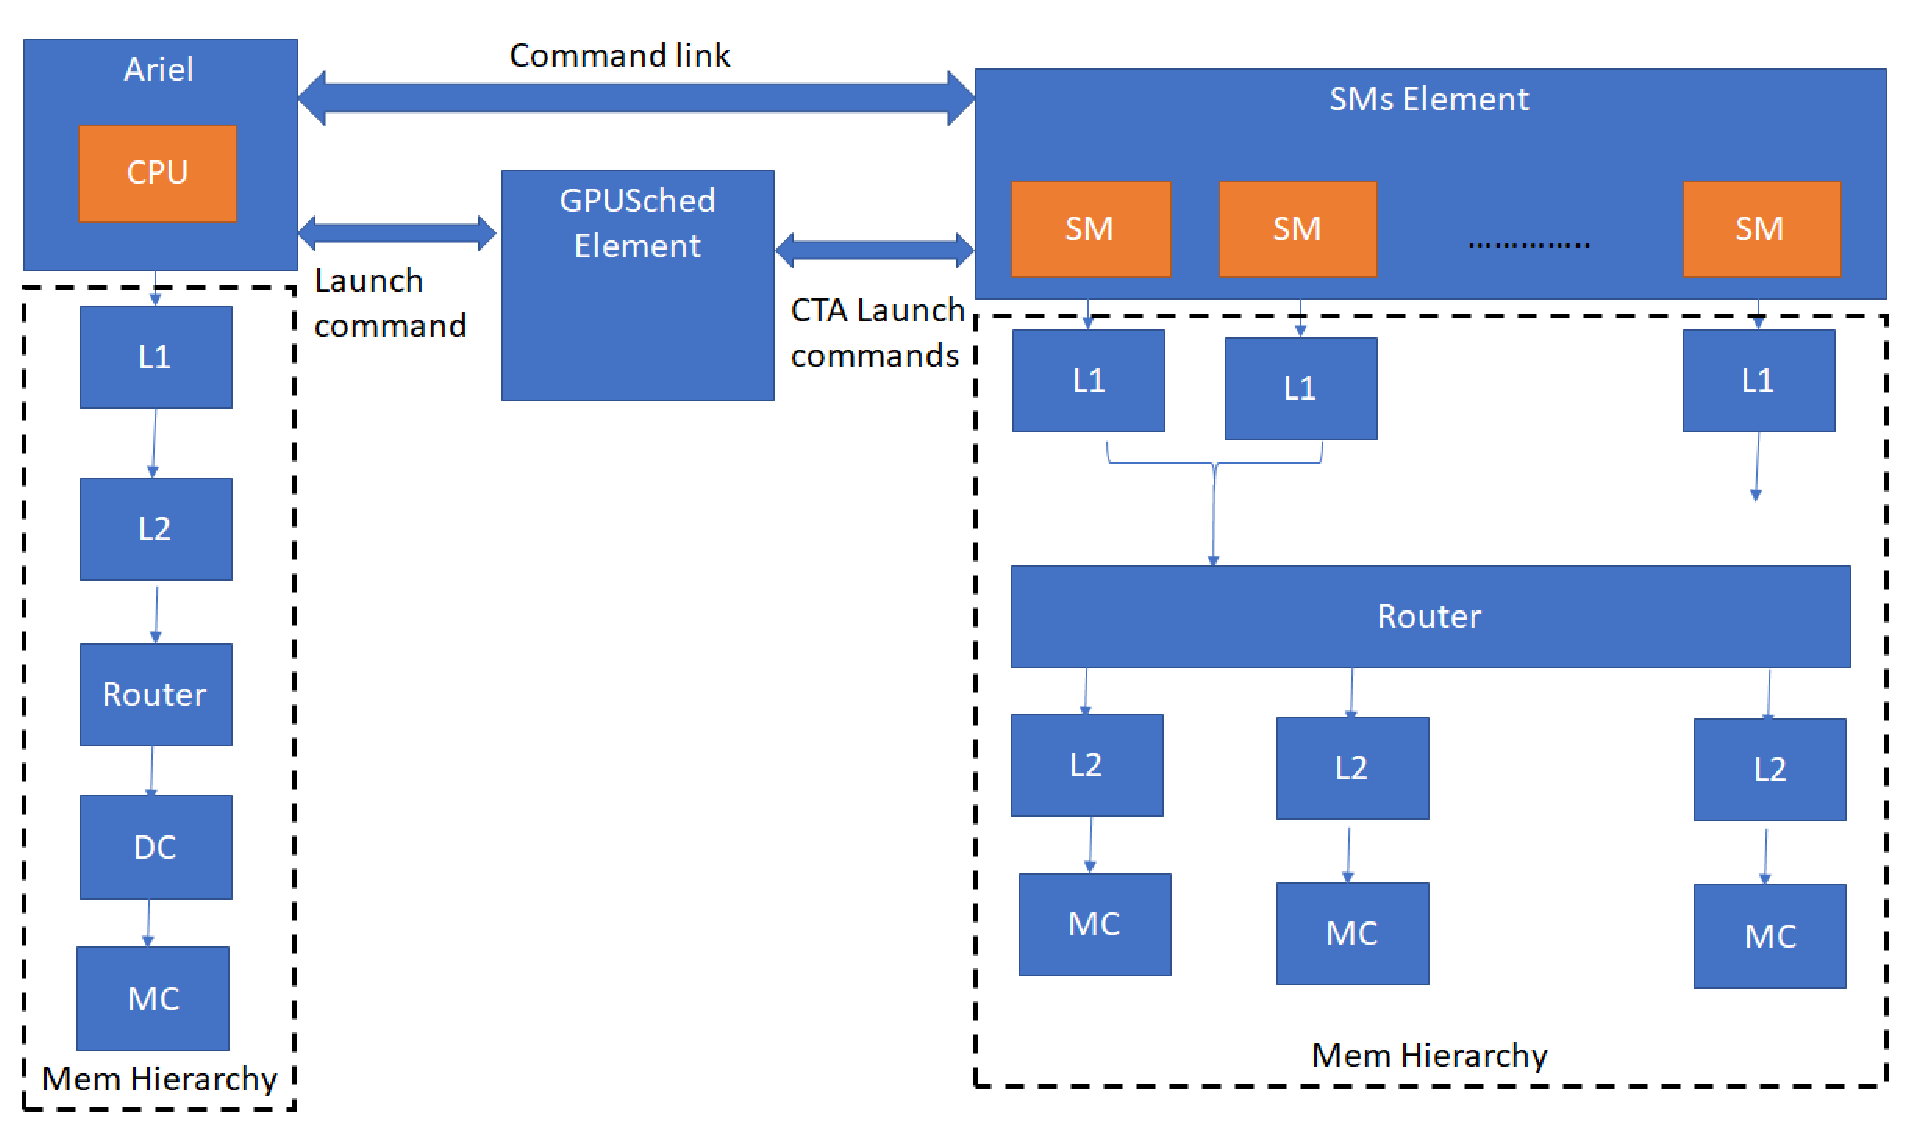
\includegraphics[width=.90\textwidth,keepaspectratio]{figures/3_1.eps}
      \captionsetup{width=.75\textwidth}
      \caption{Timing and memory model for SMs component}
      \label{fig:gpu_mem_model}
   \end{figure}
